Currently the environments that are simulated with head mounted devices do not support a lot of movement.
This is mainly because users would need a large empty room or the developers only can create small virtual environments.
So a lot of research is done to decrease the space users need to feel like they are really walking in a big virtual environment, while actually moving in a small room.
This can be done by decreasing or increasing the angle when people are rotating.
While doing this, the users feels like he is still walking straight, but in reality he is walking in circles as shown in Figure~\ref{figprob1}.
In that way the amount of space an user need is decreased.

\begin{figure}[ht!]
\centering
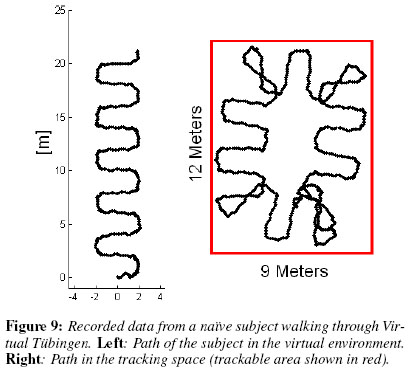
\includegraphics{sections/problem/figproblem1.jpg}
\caption{Decrease space needed by changing the angles of corners \label{figprob1}}
\end{figure}

The perceived reality by the users depends mostly on the user.
We can really decrease or increase the angle to minimize the space needed, but then the user does not perceive the virtual environment as real anymore.
So we need to find the points at which the user still perceives the virtual environment as real, but minimizes the space needed.

So the goal of our project is:
We would like to minimize the space needed to walk the path that is shown in the virtual environment, while users still perceive that they actually walked the path in the virtual environment.
